%!TEX root = ../main.tex

\section{Численное исследование}

\subsection{Улучшенная оценка устойчивости}

В предыдущем разделе из анализа уравнения \eqref{eq:spectral} было получено условие \eqref{cond:spectral_0}, необходимое для устойчивости разностной схемы \eqref{sch:transition}, \eqref{sch:borders} при $\phi \approx 0$. Предположение о его полезности основано на том, что типичным поведением модели будет некоторый процесс перехода $\phi$ от $1$ к $0$ (<<разрушение>>) за конечное время, а затем бесконечно долгое пребывание в состоянии $\phi \approx 0$.

Однако проделанного анализа уравнения \eqref{eq:spectral} в точке $\phi = 0$ недостаточно. В самом деле, было использовано, что $\epsilon''(0) = 0$ (см. выражение \eqref{eq:epsilon_phi_phi}), но не учтено, что $\epsilon''(\phi)$ при малых $\delta$ вблизи $0$ растет очень быстро и достигает больших значений (рис.~\ref{fig:eps_phi_phi}). Получается, что модель, устойчивая в точке $0$, может работать неадекватно в малой ее окрестности. Это нас, конечно, не устраивает -- улучшим оценку устойчивости.

\begin{figure}[!tp]
    \centering
    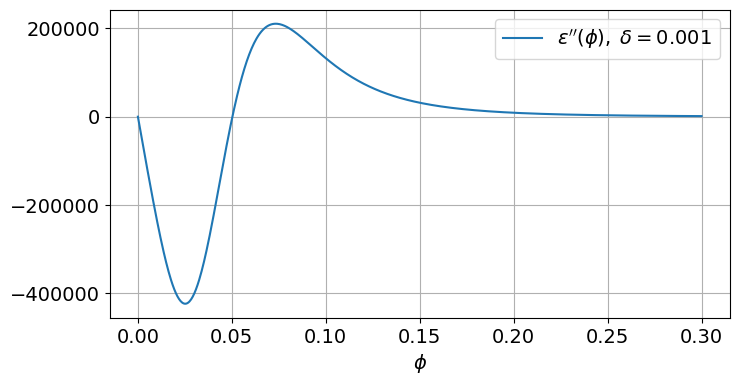
\includegraphics[width=\textwidth]{figures/eps_phi_phi.png}
    \vspace{-0.7cm}
    \caption{Поведение функции $\epsilon''(\phi)$ около $0$.}
    \label{fig:eps_phi_phi}
\end{figure}

Нужно оценить экстремумы функции $\epsilon''(\phi)$ вблизи $0$. Для начала найдем нули $\epsilon'''(\phi)$. Имеем:
$$f'''(\phi) = 24 - 72 \phi; \quad \epsilon'''_{fff} = \cfrac{-6 \epsilon_0}{(f(\phi) + \delta)^4} \tsemicolon$$
\begin{equation}
    \epsilon''' = \epsilon'''_{fff} \cdot (f')^3 + 3 \epsilon''_{ff} \cdot f' \cdot f'' + \epsilon'_f \cdot f''' = \epsilon_0 \cfrac{-6 (f')^3 + 6 (f + \delta) f' f'' - (f + \delta)^2 f'''}{(f + \delta)^4} \tpoint
    \label{eq:epsilon_phi_phi_phi}
\end{equation}
Приравняв $\epsilon'''$ к $0$, получим:
$$-6 (f')^3 + 6 (f + \delta) f' f'' - (f + \delta)^2 f''' = 0 \tcomma$$
или
\begin{multline*}
    -6(12 \phi^2 (1 - \phi))^3 + 6(4 \phi^3 - 3\phi^4 + \delta) \cdot 12 \phi^2 (1 - \phi) \cdot 12 \phi (2 - 3\phi) - \\ - (4 \phi^3 - 3 \phi^4 + \delta)^2 \cdot 24 (1 - 3 \phi) = 0 \tpoint
\end{multline*}
Разделим последнее уравнение на $24\phi^6$, получим:
$$-3 \cdot 12^2 (1 - \phi)^3 + 36 \left(4 - 3\phi + \cfrac{\delta}{\phi^3} \right)(1 - \phi)(2 - 3\phi) - \left(4 - 3 \phi + \cfrac{\delta}{\phi^3} \right)^2 (1 - 3 \phi) = 0 \tpoint$$
Пусть $\delta_n \to +0$ и корень $\phi_n \to +0$, причем $\delta_n/\phi_n^3$ ограничено. Тогда:
$$-3 \cdot 12^2 \cdot 1^3 + 36 \left(4 + \cfrac{\delta_n}{\phi_n^3} \right) \cdot 1 \cdot 2 - \left(4 + \cfrac{\delta_n}{\phi_n^3} \right)^2 \cdot 1 \to 0 \tcomma$$
$$\left(4 + \cfrac{\delta_n}{\phi_n^3} \right)^2 - 72 \left(4 + \cfrac{\delta_n}{\phi_n^3} \right) + 3 \cdot 12^2 \to 0 \tpoint$$
Значит, последовательность $4 + \delta_n/\phi_n^3$ имеет не более двух частичных пределов $\xi_+$ и $\xi_-$ -- корней уравнения $\xi^2 - 72 \xi + 432 = 0$. Первому корню $\xi_+ = 36 + 12 \sqrt{6}$ соответствует
$$\phi = \cfrac{1}{\sqrt[3]{32 + 12 \sqrt{6}}} \sqrt[3]{\delta_n} \approx \cfrac{1}{3.945} \sqrt[3]{\delta_n} \tcomma$$
второму корню $\xi_- = 36 - 12 \sqrt{6}$ соответствует
$$\phi = \cfrac{1}{\sqrt[3]{32 - 12 \sqrt{6}}} \sqrt[3]{\delta_n} \approx \cfrac{1}{1.376} \sqrt[3]{\delta_n} \tpoint$$

Из проделанного рассуждения следует, что при $\delta \to +0$ функция $\epsilon'''(\phi)$ имеет в окрестности $0$ два корня
\begin{equation}
    \phi_{\pm} = \cfrac{1}{\sqrt[3]{32 \pm 12 \sqrt{6}}} \sqrt[3]{\delta} [1 + o(1)] \tpoint
    \label{eq:epsilon_phi_phi_phi_roots}
\end{equation}

Оценим $\epsilon''(\phi)$ в точках $\phi_{\pm}$ при $\delta \to +0$. Пусть $\phi = (1/c) \sqrt[3]{\delta}, \; c \in \Real$. Тогда:
\begin{multline*}
    \cfrac{\epsilon''}{\epsilon_0} = \cfrac{2(f')^2 - (f + \delta)f''}{(f + \delta)^3} = \cfrac{2 \cdot 12^2 \phi^4 (1 - \phi)^2 - (4 \phi^3 - 3 \phi^4 + \delta) \cdot 12 \phi (2 - 3 \phi)}{(4 \phi^3 - 3 \phi^4 + \delta)^3} = \\ = \cfrac{2 \cdot 12^2 - 8 \cdot 12 - 24 (\delta/\phi^3)}{4^3 + 3 \cdot 4^3 (\delta/\phi^3) + 3 \cdot 4 (\delta/\phi^3)^2 + (\delta/\phi^3)^3} \cdot \cfrac{1}{\phi^5}[1 + o(1)] = c^5 \delta^{-5/3} \cfrac{24(8 - c^3)}{(4 + c^3)^3}[1 + o(1)] \tpoint
\end{multline*}
Отсюда:
\begin{equation}
    \epsilon''(\phi_+) \approx -4.378 \epsilon_0 \delta^{-5/3}; \quad \epsilon''(\phi_-) \approx 2.216 \epsilon_0 \delta^{-5/3} \tpoint
    \label{est:epsilon_phi_phi_bounds}
\end{equation}
Оценки экстремумов $\epsilon''(\phi)$ вблизи $0$ показаны на рис. \ref{fig:eps_phi_phi_multiplied}.

\begin{figure}[!tp]
    \centering
    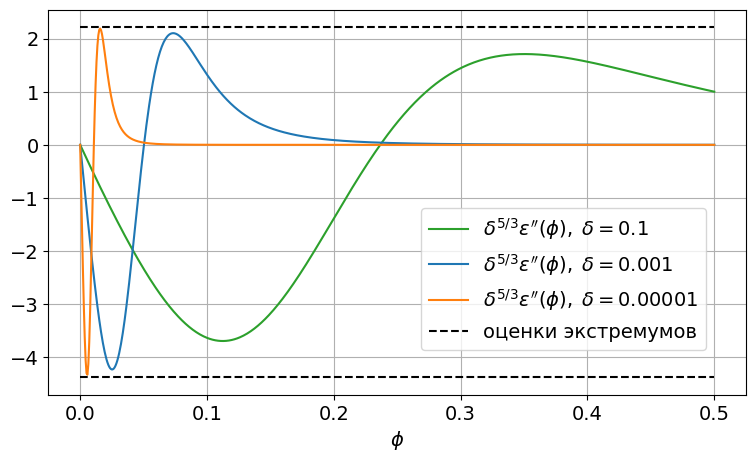
\includegraphics[width=\textwidth]{figures/eps_phi_phi_multiplied.png}
    \caption{Сравнение функций $\delta^{5/3} \epsilon''(\phi)$ при различных значениях $\delta$.}
    \label{fig:eps_phi_phi_multiplied}
\end{figure}

Получим новую оценку устойчивости, рассмотрев уравнение \eqref{eq:spectral} в точке $\phi = \phi_+$. $\epsilon''(\phi_+) \approx -4.4 \epsilon_0 \delta^{-5/3}$. Сумма в скобках отрицательна ($\delta$ мало, $\epsilon''(\phi_+)$ велико по модулю и отрицательно), поэтому $f''(\phi_0) > 0$ можно считать равным $0$: оценку это только усилит. Преобразовав уравнение \eqref{eq:spectral}, получим:
$$\lambda(\theta) = 1 + m \tau \left( -\cfrac{2.2 K_\Phi^2 \epsilon_0}{\delta^{5/3}} - \cfrac{2 \Gamma}{h^2} \sin^2 \cfrac{\theta}{2} \right) \tpoint$$
Условие $|\lambda(\theta)| \leqslant 1$ справедливо для любого $\theta$, если и только если
\begin{equation}
    \tau \leqslant \left( \cfrac{1.1 m K_\Phi^2 \epsilon_0}{\delta^{5/3}} + \cfrac{m \Gamma}{h^2} \right)^{-1} \tpoint
    \label{cond:spectral_better_theoretical}
\end{equation}

Для применения на практике оценку \eqref{cond:spectral_better_theoretical} нужно брать <<с запасом>> (экспериментальное обоснование будет дано позже). Сделаем оценку строже, примерно удвоив знаменатель:
\begin{equation}
    \tau \leqslant \cfrac{1}{2m} \left( \cfrac{K_\Phi^2 \epsilon_0}{\delta^{5/3}} + \cfrac{\Gamma}{h^2} \right)^{-1} \tpoint
    \label{cond:spectral_better}
\end{equation}

Более простая оценка не слабее оценки \eqref{cond:spectral_better} выглядит следующим образом:
\begin{equation}
    \tau \leqslant \cfrac{1}{4m} \min \left(\cfrac{\delta^{5/3}}{K_\Phi^2 \epsilon_0}, \; \cfrac{h^2}{\Gamma} \right) \tpoint
    \label{cond:spectral_better_simpler}
\end{equation}

Полученная оценка \eqref{cond:spectral_better} устойчивости разностной схемы \eqref{sch:transition}, \eqref{sch:borders} содержит все параметры уравнения \eqref{eq:one_dim_simpler}, кроме $l$.


\subsection{Вычислительный эксперимент: устойчивость}

Была написана программа, реализующая разностную схему \eqref{sch:transition}, \eqref{sch:borders}. Проверим на практике устойчивость и сходимость.

Зафиксируем параметры уравнения \eqref{eq:one_dim_simpler}:
\begin{equation}
    \epsilon_0 = 0.2, \; \delta = 0.04, \; l = 1.0, \; \Gamma = 1.0, \; m = 0.5, \; K_\Phi = 4.8 \tpoint
    \label{exp:parameters}
\end{equation}
Отметим, что перед нами случай <<сильного напряжения>> (см. выражение \eqref{char:equilibriums}).

Моделируем решение в области 
\begin{equation}
    \Omega = [0, w]_x \times [0, T]_t, \; w = 5, \; T = 1 \tpoint
    \label{exp:set}
\end{equation}

Зададим следующие краевые условия:
\begin{equation}
\begin{gathered}
    \phi(0, t) = 1, \; \phi(w, t) = 1 \tcomma \\
    \phi(x, 0) \equiv \phi_0(x) = \begin{cases}
        1, \; \text{если} \; x \leqslant 2.25 \; \text{или} \; x \geqslant 2.75 \tsemicolon \\
        1 - 0.025 \cdot [1 + \cos(4 \pi x)], \; \text{если} \; 2.25 < x < 2.75 \tpoint
    \end{cases}
\end{gathered} \label{exp:borders}
\end{equation}
Обратим внимание, что $\phi_0(x)$ дважды дифференцируема всюду, кроме конечного числа точек, с ограниченной второй производной.

Обозначим $n_x$ количество отрезков разбиения $[0, w]_x$ (узлов, соответственно, $n_x + 1$); $n_t$ -- количество отрезков разбиения $[0, T]_t$. $h = w/n_x, \; \tau = T/n_t$.

\begin{figure}[!tp]
    \centering
    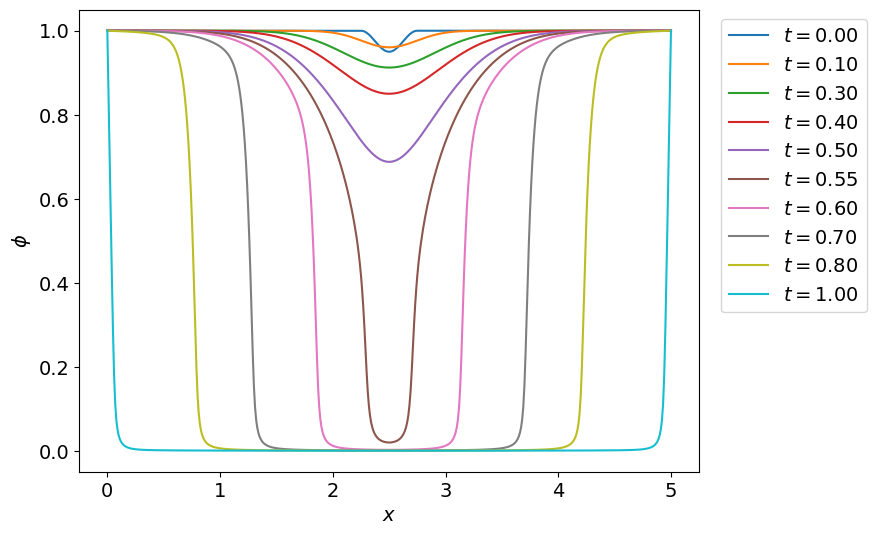
\includegraphics[width=\textwidth]{figures/typical_solution.png}
    \vspace{-0.8cm}
    \caption{Типичное решение задачи, $n_x = 10^3, \; n_t = 10^5$.}
    \label{fig:typical_solution}
\end{figure}

Для начала посмотрим на типичное решение исследуемой задачи (рис. \ref{fig:typical_solution}). Видно постепенное развитие канала электрического пробоя (разрушение среды) из небольшого начального возмущения фазового поля $\phi$ неповрежденной среды. Примерно в момент времени $t = 0.55$ канал пробоя <<прорастает насквозь>>, а именно, $\phi$ вблизи точки $x = 2.5$ приближается к нулевому значению. Обратим внимание, что в период времени $t \in (0.3, \; 0.55)$ канал пробоя (область, где $\phi$ существенно отличается от $1$) практически не растет в ширину, а при $t > 0.55$, напротив, растет в ширину почти с постоянной скоростью.

Проверим полученную в предыдущем разделе оценку \eqref{cond:spectral_better} устойчивости разностной схемы. Будем считать, что в вычислительном эксперименте схема неустойчива, если программа завершилась с ошибкой: произошло деление на $0$ (в формуле \eqref{eq:epsilon} функции $\epsilon(\phi)$ при $f(\phi) = -\delta$) или значения $\phi$ ушли на бесконечность (переполнился тип double). Будем перебирать $n_x$ и $n_t$, запоминая пары соседних точек, в одной из которых устойчивость есть, а в другой нет. Так получим опытную оценку устойчивости схемы. Отобразим ее на графике вместе с оценкой \eqref{cond:spectral_better} (рис. \ref{fig:stability_bounds}).

Эксперимент показывает, что оценка \eqref{cond:spectral_better} удачна: она примерно повторяет контур опытной оценки, к тому же ее график лежит выше, то есть она имеет некоторый <<запас>> до момента, когда в программе возникает ошибка. Именно ради этого <<запаса>> знаменатель исходной оценки  \eqref{cond:spectral_better_theoretical} был удвоен.

\begin{figure}[!tp]
    \centering
    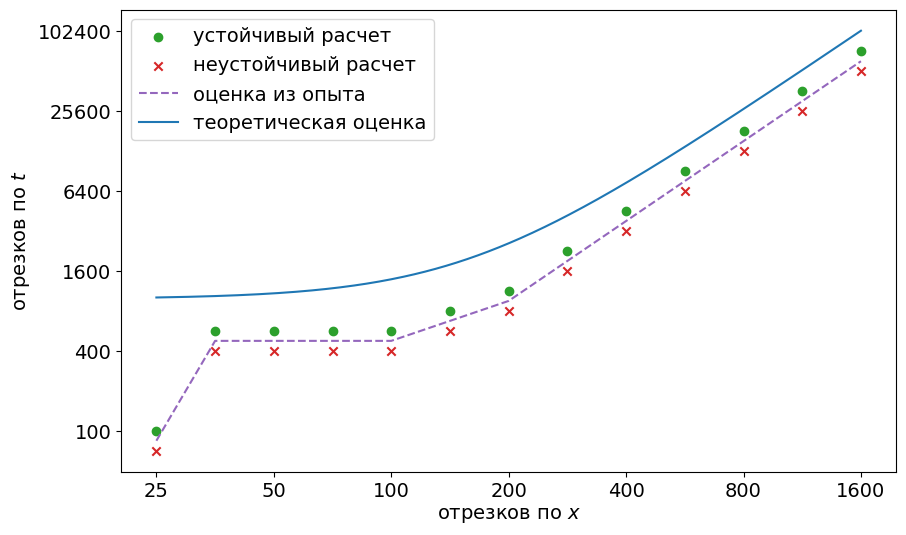
\includegraphics[width=\textwidth]{figures/stability_bounds.png}
    \vspace{-0.7cm}
    \caption{Теоретическая и опытная оценки устойчивости разностной схемы.}
    \label{fig:stability_bounds}
\end{figure}


\subsection{О сходимости решения разностной задачи}

Если разностная схема аппроксимирует задачу Коши и к тому же обладает устойчивостью при заданной связи $\tau =\tau(h)$, то решение разностной задачи сходится к решению задачи Коши при $h \to 0$.

Расшифруем перечисленные понятия более формально.

Пусть $\Omega \subset \Real^s$ -- пространство независимых переменных, $\Gamma = \partial \Omega$ -- граница $\Omega$, $\Int \Omega = \Omega \smallsetminus \partial \Omega$ -- внутренность $\Omega$; задан класс $Y$ функций $y(\vx)$ на $\Omega$ (обладающих некоторыми содержательными свойствами, например, гладкостью).

Задан оператор $R: Y \longrightarrow I$, где $I$ -- некоторое пространство функций на $\Int \Omega$; задан оператор $r: Y \longrightarrow G$, где $G$ -- некоторое пространство функций на $\partial \Omega$. $R$ и $r$ не обязательно линейные; подразумевается, что они включают в себя операции дифференцирования. Сформулируем дифференциальную задачу:
\begin{equation}
    \{ \quad Ry = 0; \quad ry = 0 \quad \} \tpoint
    \label{eq:formal_differential}
\end{equation}
Здесь $y(\vx) \in Y$ -- искомая функция. Первое уравнение имеет смысл условия на $y$ во внутренности $\Omega$, второе -- краевого условия.

В пространстве $\Omega$ введем сетку, то есть определим некоторое конечное подмножество $\Omega_h \subset \Omega$. Здесь $h$ -- параметр, имеющий смысл мелкости шага сетки, -- то есть, строго говоря, определено семейство сеток. Функцию $y \in Y$ можно ограничить на $\Omega_h$ -- введем обозначение $[y]_h = y|_{\Omega_h}$. Пусть $Y_h = \{[y]_h: y \in Y\}, \; I_h = \{[i]_h: i \in I\}, \; G_h = \{[g]_h: g \in G\}$. Некоторые $R_h: Y_h \longrightarrow I_h$ и $r_h: Y_h \longrightarrow G_h$ будем называть разностными операторами. Теперь можно сформулировать разностную задачу:
\begin{equation}
    \{ \quad R_h y_h = 0; \quad r_h y_h = 0 \quad \} \tpoint
    \label{eq:formal_subtractive}
\end{equation}
$y_h \in Y_h$ -- искомая сеточная функция.

Пусть на пространствах $Y$, $I$, $G$ определены некоторые нормы $\| \cdot \|_Y$, $\| \cdot \|_I$, $\| \cdot \|_G$ соответственно. Пусть на пространстве $Y_h$ определена норма $\| \cdot \|_{Y_h}$, такая что $\forall y \in Y \; \| \, [y]_h \, \|_{Y_h} \to \| \, y \, \|_Y$ при $h \to 0$. В этом случае нормы $\| \cdot \|_Y$ и $\| \cdot \|_{Y_h}$ назовем \emph{согласованными}. Пусть аналогично $\| \cdot \|_{I_h}$ и $\| \cdot \|_{G_h}$ -- нормы на $I_h$ и $G_h$, согласованные с $\| \cdot \|_I$ и $\| \cdot \|_G$ соответственно.

Теперь можно формально определить аппроксимацию, устойчивость и сходимость.

Разностная задача \eqref{eq:formal_subtractive} \emph{аппроксимирует} дифференциальную задачу \eqref{eq:formal_differential}, если
$$\forall y \in Y \quad \| \, [Ry]_h - R_h [y]_h \, \|_{I_h} + \| \, [ry]_h - r_h [y]_h \, \|_{G_h} \to 0 \text{ при } h \to 0 \tpoint$$
Порядок $k$ стремления выражения к $0$ по $h$ называют порядком аппроксимации.

Решение $y_h$ разностной задачи \eqref{eq:formal_subtractive} \emph{сходится} к решению $y$ дифференциальной задачи \eqref{eq:formal_differential}, если
$$\| \, [y]_h - y_h \, \|_{Y_h} \to 0 \text{ при } h \to 0 \tpoint$$
Порядок $k$ стремления выражения к $0$ по $h$ называют порядком сходимости.

Разностная задача \eqref{eq:formal_subtractive} \emph{устойчива}, если
$$\exists M \in \Real \; \forall h \; \forall y_h, z_h \in Y_h \quad \| \, y_h - z_h \, \|_{Y_h} \leqslant M \cdot (\| \, R_h y_h - R_h z_h \, \|_{I_h} + \| \, r_h y_h - r_h z_h \, \|_{G_h}) \tpoint$$

Легко видеть, что из аппроксимации и устойчивости следует сходимость. Пусть $y$ -- решение задачи \eqref{eq:formal_differential}, $y_h$ -- решение задачи \eqref{eq:formal_subtractive}. Запишем неравенство из определения устойчивости, положив $z_h = [y]_h$:
$$\| \, y_h - [y]_h \, \|_{Y_h} \leqslant M \cdot (\| \, R_h y_h - R_h [y]_h \, \|_{I_h} + \| \, r_h y_h - r_h [y]_h \, \|_{G_h}) \tpoint$$
$y_h$ -- решение разностной задачи, следовательно, $R_h y_h \equiv 0, \; r_h y_h \equiv 0$. $y$ -- решение дифференциальной задачи, $Ry \equiv 0, \; ry \equiv 0$, а значит, $[Ry]_h \equiv 0, \; [ry]_h \equiv 0$. Вычтя и прибавив нулевые слагаемые, получим:
$$\| \, y_h - [y]_h \, \|_{Y_h} \leqslant M \cdot (\| \, [Ry]_h - R_h [y]_h \, \|_{I_h} + \| \, [ry]_h - r_h [y]_h \, \|_{G_h}) \tpoint$$
В правой части неравенства выражение из определения аппроксимации, стремящееся к~$0$. В итоге $\| \, [y]_h - y_h \, \|_{Y_h} \to 0$ -- доказана сходимость. Отметим, что порядок сходимости $k$ в таком случае совпадает с порядком аппроксимации.

Приведенные построения могут быть непосредственно применены к разностной схеме, описанной в разделе \ref{sec:differential_scheme}, тем самым доказывая ее сходимость.


\subsection{Вычислительный эксперимент: сходимость}

Аппроксимация схемой \eqref{sch:transition}, \eqref{sch:borders} задачи Коши \eqref{eq:one_dim_simpler}, \eqref{eq:cauchy_borders} очевидна; для устойчивости схемы получено условие \eqref{cond:spectral_better}, строго говоря, являющееся лишь необходимым, но применимое на практике. Теперь экспериментально проверим сходимость.

Поясним связь формальных конструкций предыдущего раздела с решаемой задачей Коши.

На множестве $C_2(\Omega)$ дважды непрерывно дифференцируемых функций в замкнутой области $\Omega = [0, w]_x \times [0, T]_t$ рассмотрим следующие нормы: непрерывную $\| \cdot \|_C$ и $L_2$-норму $\| \cdot \|_2$.
$$\| \, f \, \|_C = \max \limits_{(x, t) \in \Omega} f(x, t); \qquad \| \, f \, \|_{2} = \sqrt{\int \limits_{\Omega} f^2(x, t) dx dt} \tpoint$$
Эти же нормы введем на множествах $C(\partial \Omega)$ и $C(\Int \Omega)$ непрерывных функций на границе и внутренности $\Omega$ соответственно.

Теперь рассмотрим регулярную сетку $\Omega_{h, \tau}$; введем некоторую зависимость $\tau = \tau(h)$. Ограничивая функции из $C_2(\Omega)$, $C(\Int \Omega)$ и $C(\partial \Omega)$ на множестве $\Omega_h = \Omega_{h, \tau(h)}$, получаем множества $C_2(\Omega)_h$, $C(\Int \Omega)_h$ и $C(\partial \Omega)_h$ сеточных функций.

На перечисленных множествах сеточных функций введем нормы, согласованные с $\| \cdot \|_C$ и $\| \cdot \|_2$:
$$\| \, f_a^b \, \|_C = \max \limits_{(a, b) \in \Omega_h} f_a^b; \qquad \| \, f_a^b \, \|_2 = \sqrt{\cfrac{1}{h \tau}\sum \limits_{(a, b) \in \Omega_h} (f_a^b)^2} \tpoint$$

Задачу Коши \eqref{eq:one_dim_simpler}, \eqref{eq:cauchy_borders} легко привести к виду \eqref{eq:formal_differential}, где $R: C_2(\Omega) \longrightarrow C(\Int \Omega)$, $r: C_2(\Omega) \longrightarrow C(\partial \Omega)$; разностную задачу \eqref{sch:transition}, \eqref{sch:borders} -- к виду \eqref{eq:formal_subtractive}, где $R_h: C_2(\Omega)_h \longrightarrow C(\Int \Omega)_h$, $r_h: C_2(\Omega)_h \longrightarrow C(\partial \Omega)_h$.

Перейдем к вычислительному эксперименту. Сходимость будем проверять по описанным выше нормам $\| \cdot \|_C$ и $\| \cdot \|_2$ на множестве сеточных функций. Так как аналитическое решение задачи Коши не известно, будем сравнивать ряд результатов на все более мелких сетках по норме с лучшим результатом в ряду. При сравнении функцию на более мелкой сетке ограничиваем на более крупной, игнорируя часть узлов.

Зафиксируем ранее использовавшиеся параметры уравнения \eqref{exp:parameters}, \eqref{exp:set}; зададим краевые условия \eqref{exp:borders}. Положим $n_x = w / h$ -- число отрезков разбиения по $x$, $n_t = T / \tau$ -- по $t$.

Во всех описанных далее вариантах расчетов соблюдается условие устойчивости~\eqref{cond:spectral_better}.

Для начала зафиксируем $n_x = 200$ и будем перебирать $n_t$, каждый раз увеличивая его вдвое. Сравнение по нормам с результатом при $n_t = 204800$ изображено на рис. \ref{fig:convergence_fixed_nx}. Разностная схема имеет первый порядок аппроксимации по $t$; опыт показывает первый порядок сходимости ошибки $O(\tau)$.

Зафиксируем $n_t = 204800$ и будем перебирать $n_x$, каждый раз увеличивая его вдвое. Сравнение по нормам с результатом при $n_x = 1600$ изображено на рис. \ref{fig:convergence_fixed_nt}. Разностная схема имеет второй порядок аппроксимации по $x$; опыт показывает второй порядок сходимости ошибки $O(h^2)$.

\begin{figure}[!tp]
    \centering
    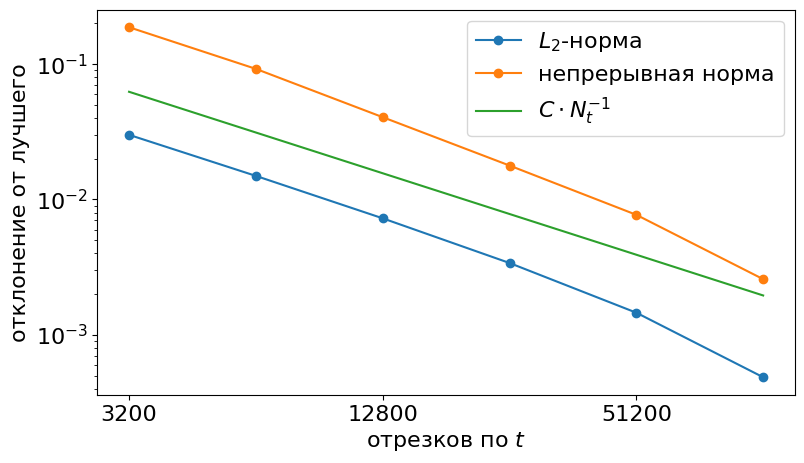
\includegraphics[width=0.72\textwidth]{figures/convergence_fixed_nx.png}
    \vspace{-0.2cm}
    \caption{Ошибка решения по норме при фиксированном $n_x = 200$.}
    \label{fig:convergence_fixed_nx}
    \vspace{0.6cm}
    
    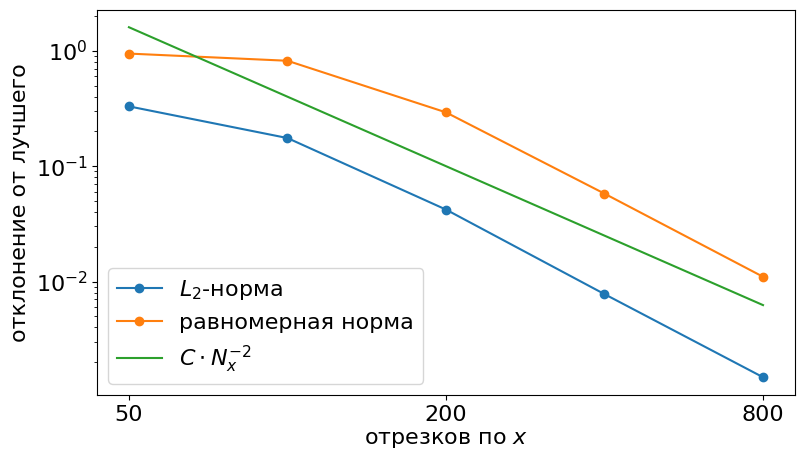
\includegraphics[width=0.72\textwidth]{figures/convergence_fixed_nt.png}
    \vspace{-0.2cm}
    \caption{Ошибка решения по норме при фиксированном $n_t = 204800$.}
    \label{fig:convergence_fixed_nt}
    \vspace{0.6cm}
    
    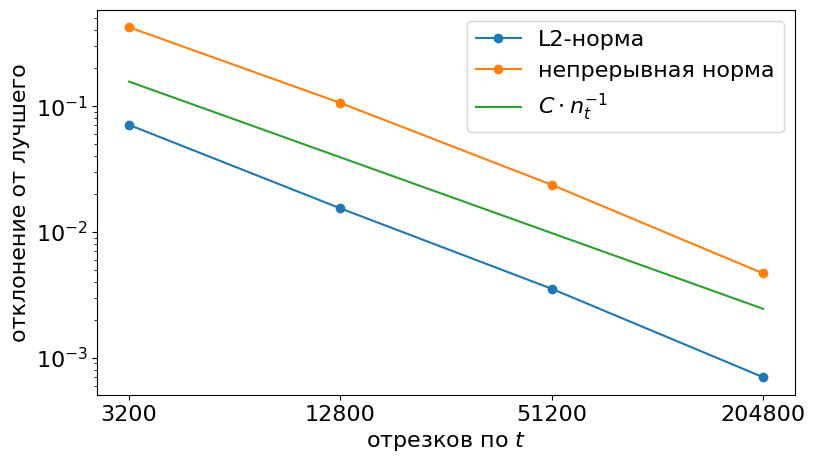
\includegraphics[width=0.72\textwidth]{figures/convergence_connected.png}
    \vspace{-0.2cm}
    \caption{Ошибка решения по норме при $n_t = 0.08 \cdot n_x^2$.}
    \label{fig:convergence_connected}
\end{figure}

Теперь свяжем $n_x$ и $n_t$ уравнением, так чтобы при $h, \tau \to 0$ выполнялось условие устойчивости \eqref{cond:spectral_better}. При выбранных параметрах модели подойдет $n_t = 0.08 \cdot n_x^2$. Аналогично проведем сравнение ряда измерений по норме с лучшим (рис. \ref{fig:convergence_connected}). Как и ожидалось, измерения показывают сходимость $O(\tau + h^2) = O(\tau)$ первого порядка по времени при выбранном уравнении связи.

В первых двух опытах, без стремления обоих шагов сетки к $0$, последовательности сеточных функций имели неясный предел. В третьем же, если принять предположение об устойчивости разностной схемы, сеточные функции сходятся к решению задачи Коши \eqref{eq:one_dim_simpler}, \eqref{eq:cauchy_borders}.


\subsection{Вычислительный эксперимент: положения равновесия}

Ранее были исследованы положения равновесия уравнения \eqref{eq:one_dim_simpler} вида $\phi \equiv C$. Их количество и устойчивость определяется значением выражения \eqref{char:equilibriums} (обозначено $\xi$). Проверим этот результат экспериментально.

Зададим модели параметры \eqref{exp:parameters}, \eqref{exp:set}. В качестве начального условия берем возмущенное положение равновесия: $\phi(x, 0) = C + A \cos(\omega x); \; \phi(0, t) \equiv \phi(0, 0), \; \phi(w, t) \equiv \phi(w, 0)$. Амплитуда $A$ мала, порядка $0.01$. $n_x = 800, \; n_t = 51200$.

Если положение равновесия устойчиво, то при любом $\omega$ возмущение угасает; если неустойчиво, то существует некоторое $\omega_0$, такое что при $\omega < \omega_0$ возмущение растет.

Положим $K_{\Phi, 1} = 0, \; K_{\Phi, 2} = 1.1, \; K_{\Phi, 3} = 4.8$. Как было сказано выше, $\delta = 0.04$. В таком случае $\xi_1 = 0 < \delta^2, \; \xi_2 = 0.121 \in (\delta^2, (1 + \delta)^2), \; \xi_3 = 2.304 > (1 + \delta)^2$.

Вначале рассмотрим $K_{\Phi, 1} = 0, \; \xi_1 < \delta^2$ -- случай слабого электрического напряжения. Система имеет два положения равновесия: $\phi \equiv 0$ неустойчивое, $\phi \equiv 1$ устойчивое. На рис. \ref{fig:equilibrium_1_0}, \ref{fig:equilibrium_1_1} видно теоретически предсказанное поведение возмущенной среды: при $C = 0$ возмущение растет, при $C = 1$ -- затухает. В точке $C = 0$ производная функции $\chi(\phi)$ (см. выражение \eqref{eq:equilibruim_characteristic}) равна $0$, поэтому, чтобы увидеть рост возмущения, приходится брать небольшое $\omega$, обеспечивая небольшое значение $\partial^2 \phi / \partial x^2$. В эксперименте с $\phi \equiv 1$ взято $C = 1 - A$, чтобы значения $\phi$ не превосходили $1$.

\begin{figure}[!t]
    \centering
    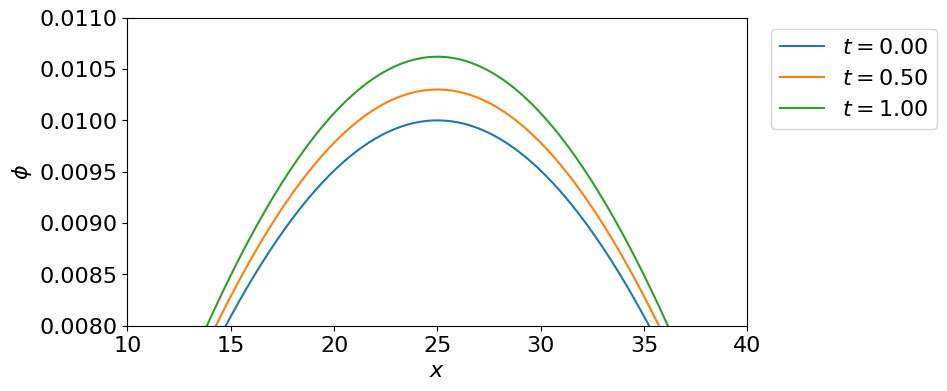
\includegraphics[width=0.9\textwidth]{figures/equilibrium_1_0.png}
    \vspace{-0.3cm}
    \caption{Случай слабого напряжения: возмущенное положение равновесия $\phi \equiv 0$, неустойчивое.}
    \label{fig:equilibrium_1_0}
    \vspace{0.5cm}
    
    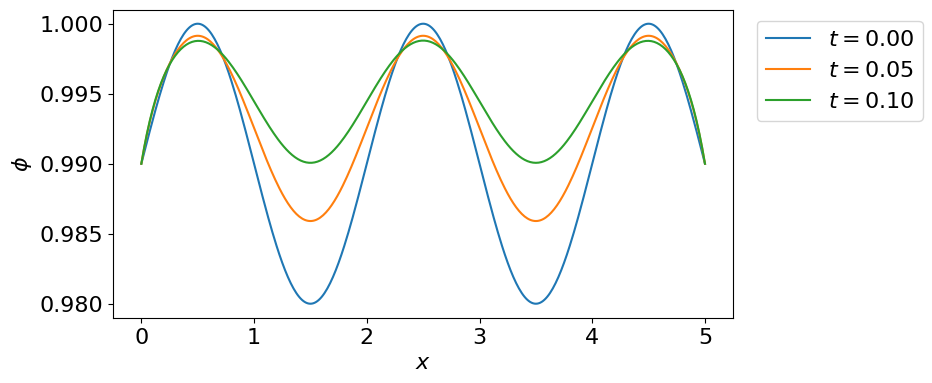
\includegraphics[width=0.9\textwidth]{figures/equilibrium_1_1.png}
    \vspace{-0.3cm}
    \caption{Случай слабого напряжения: возмущенное положение равновесия $\phi \equiv 1$, устойчивое.}
    \label{fig:equilibrium_1_1}
\end{figure}

Теперь рассмотрим $K_{\Phi, 2} = 1.1, \; \xi_2 \in (\delta^2, (1 + \delta)^2)$ -- случай среднего напряжения. Система имеет три положения равновесия: $\phi \equiv 0$ устойчивое, $\phi \equiv C_3 \approx 0.5$ неустойчивое ($C_3$ -- корень функции $\chi(\phi)$ в интервале $(0, 1)$), $\phi \equiv 1$ устойчивое. Поведение возмущенной среды изображено на рис. \ref{fig:equilibrium_2_0}, \ref{fig:equilibrium_2_05}, \ref{fig:equilibrium_2_1}, оно соответствует теоретическим результатам.

\begin{figure}[!tp]
    \centering
    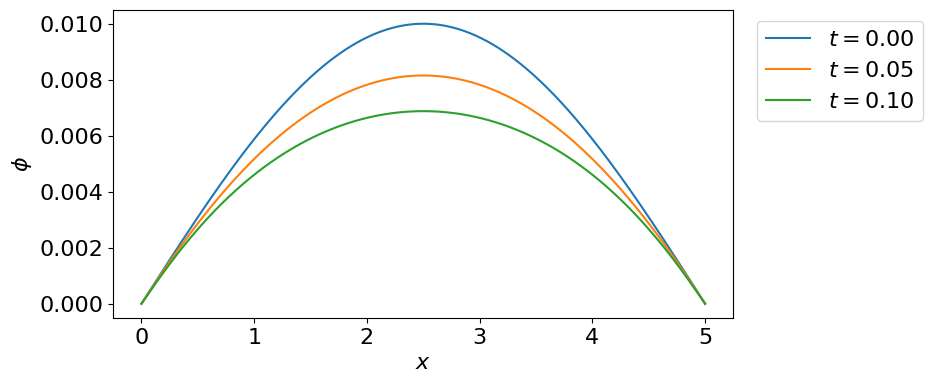
\includegraphics[width=0.9\textwidth]{figures/equilibrium_2_0.png}
    \vspace{-0.3cm}
    \caption{Случай среднего напряжения: возмущенное положение равновесия $\phi \equiv 0$, устойчивое.}
    \label{fig:equilibrium_2_0}
    \vspace{0.5cm}

    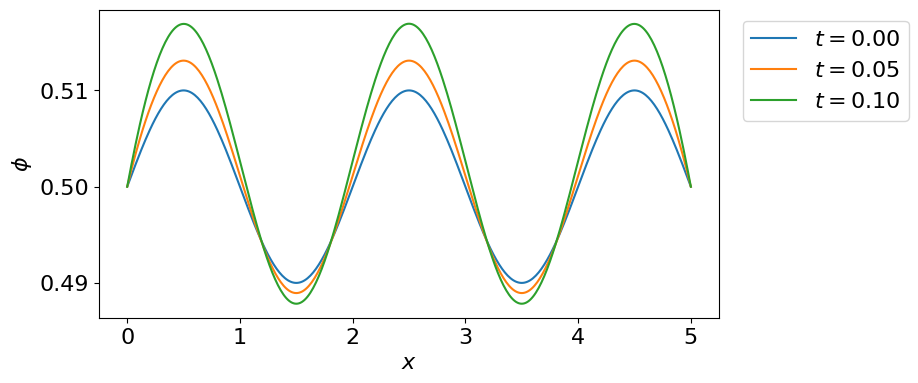
\includegraphics[width=0.9\textwidth]{figures/equilibrium_2_05.png}
    \vspace{-0.3cm}
    \caption{Случай среднего напряжения: возмущенное положение равновесия $\phi \equiv C_3 \approx 0.5$, неустойчивое.}
    \label{fig:equilibrium_2_05}
    \vspace{0.5cm}
    
    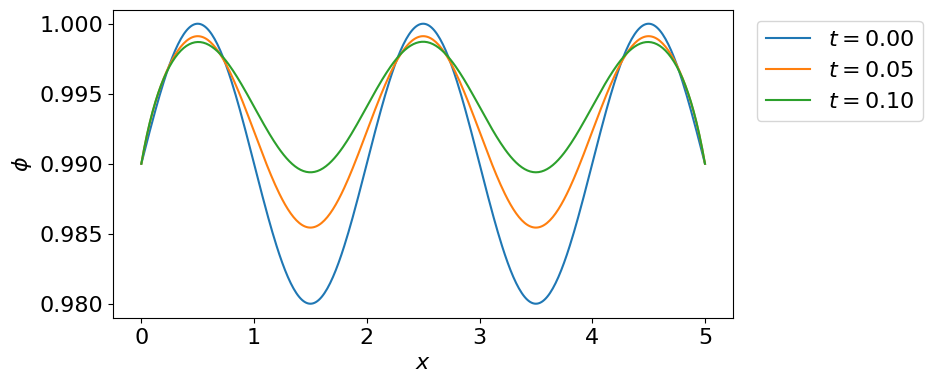
\includegraphics[width=0.9\textwidth]{figures/equilibrium_2_1.png}
    \vspace{-0.3cm}
    \caption{Случай среднего напряжения: возмущенное положение равновесия $\phi \equiv 1$, устойчивое.}
    \label{fig:equilibrium_2_1}
\end{figure}

Наконец, рассмотрим $K_{\Phi, 3} = 4.8, \; \xi_3 > (1 + \delta)^2$ -- случай сильного напряжения. Система имеет два положения равновесия: $\phi \equiv 0$ устойчивое, $\phi \equiv 1$ неустойчивое. Поведение возмущенной среды изображено на рис. \ref{fig:equilibrium_3_0}, \ref{fig:equilibrium_3_1}, оно также соответствует теории.

\begin{figure}[!t]
    \centering
    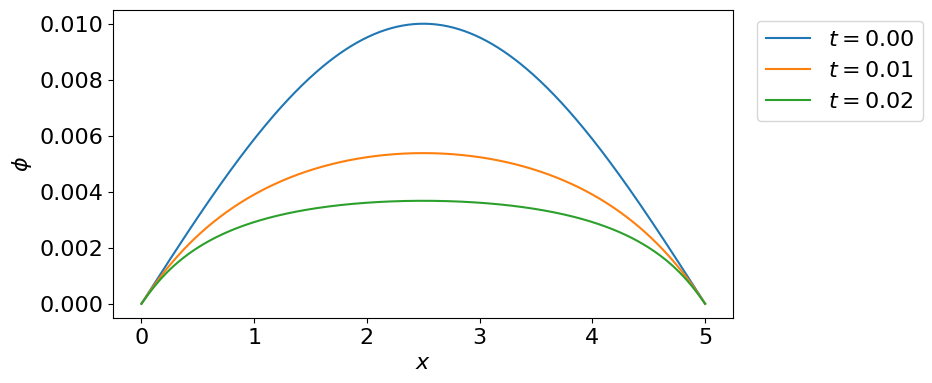
\includegraphics[width=0.9\textwidth]{figures/equilibrium_3_0.png}
    \vspace{-0.3cm}
    \caption{Случай сильного напряжения: возмущенное положение равновесия $\phi \equiv 0$, устойчивое.}
    \label{fig:equilibrium_3_0}
    \vspace{0.5cm}
    
    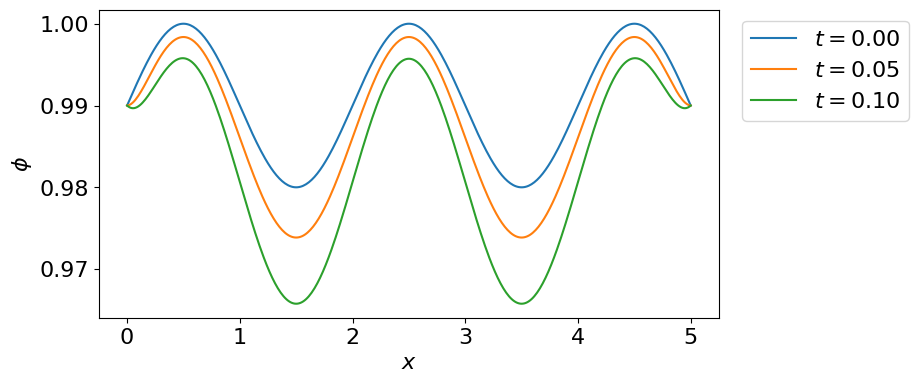
\includegraphics[width=0.9\textwidth]{figures/equilibrium_3_1.png}
    \vspace{-0.3cm}
    \caption{Случай сильного напряжения: возмущенное положение равновесия $\phi \equiv 1$, неустойчивое.}
    \label{fig:equilibrium_3_1}
\end{figure}